
%%%%%%%%%%%%%%%%%%%%%%%%%%%%%%%%%%%%%%%%%%%%%%%%%%%%%%%%%%%
%% Capítulo 2: Polinomios Ortoganles Clásicos            %%
%%%%%%%%%%%%%%%%%%%%%%%%%%%%%%%%%%%%%%%%%%%%%%%%%%%%%%%%%%%


En el capítulo \ref{chap:introduccionPO} hemos mostrado una amplia introducción a la ortogonalidad y presentado ejemplos concretos de polinomios ortogonales. En este capítulo presentaremos las familias concretas de polinomios ortogonales más importantes: los \textit{polinomios ortogonales clásicos}. Estos son los polinomios de Hermite, Laguerre, Jacobi y Bessel. Estas familias presentan la peculiaridad de ser las únicas que verifican ciertas propiedades, entre las que destaca la \textit{ecuación diferencial de Pearson}. Estos polinomios, entre otras disciplinas pueden ser encontrados en problemas de Sturm-Liouville cuando se utilizan ecuaciones diferenciales hipergeométricas.

\begin{figure}[h]
    \centering
    \begin{tabular}{ccc}
        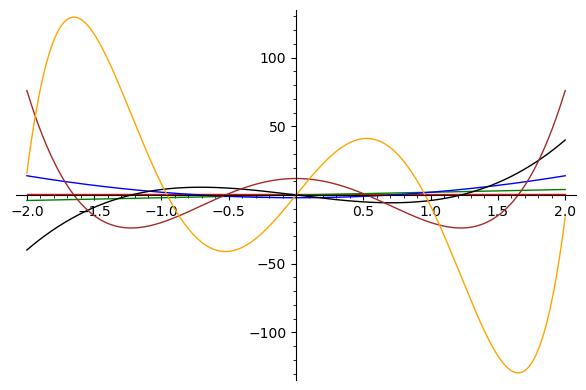
\includegraphics[width=5cm]{img/C2/hermite.png} & 
        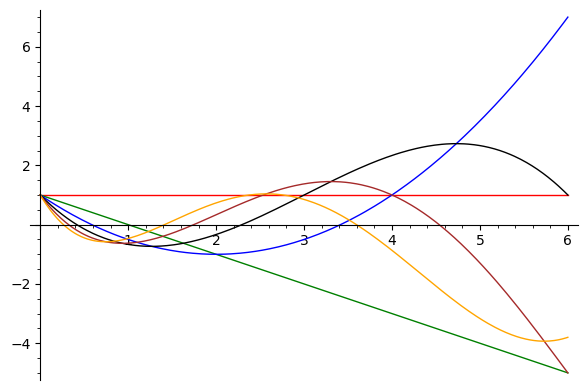
\includegraphics[width=5cm]{img/C2/laguerre.png} &
        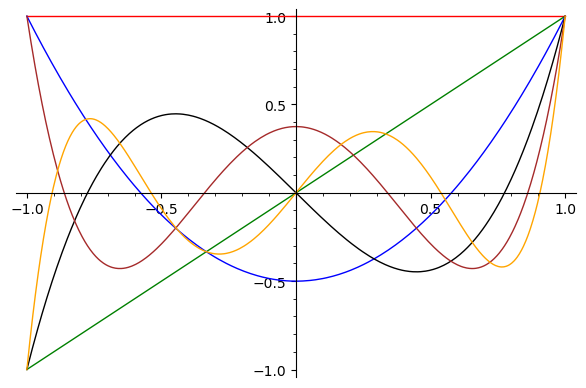
\includegraphics[width=5cm]{img/C2/jacobi.png} \\
        (a) Hermite $H_n$ & (b) Laguerre $L^{(0)}_n$ & (c) Jacobi $J^{(0,0)}_n$ 
    \end{tabular}
    \caption{Polinomios Ortogonales Clásicos}
    \label{img:graficas-clasicos}
\end{figure}

En las imágenes \ref{img:graficas-clasicos} podemos ver la representación gráfica, para parámetros concretos que definiremos próximamente, de los polinomios ortogonales de Hermite, Laguerre y Jacobi. Estas tres son las familias que mayor atención recibirán de nuestra parte al ser aquellas cuya ortogonalidad se manifiesta en intervalos reales.

\section{La ecuación de Pearson}

Para empezar, introduciremos una nueva notación para los funcionales de momentos que también se suele utilizar. Sea $\uu$ un funcional de momentos y $\{\mu_n\}$ su sucesión de momentos, entonces denotamos
\begin{equation}
    \label{eq:nueva-notacion-funcional}
    \begin{split}
        \uu:\mathbb P & \longrightarrow \R \\
        x^n & \longmapsto \left\langle \uu, x^n \right\rangle = \mu_n
    \end{split}
\end{equation}

A lo largo de este capítulo denotaremos como $\prodesc{\uu}{\pi(x)}$ a la aplicación del funcional $\uu$ a un polinomio $\pi(x)$.

Definimos a continuación dos operadores que actuán sobre los funcionales.

\begin{definicion}[Producto por un polinomio]
    Para cada polinomio $\pi$, definimos un nuevo funcional de momentos a partir de $\uu$ como
    \begin{equation}
        \begin{split}
            \pi\uu:\mathbb P & \longrightarrow \R \\
            \phi & \longmapsto \prodesc{\pi\uu}{\phi}=\prodesc{\uu}{\pi\phi}
        \end{split}
    \end{equation}
    
\end{definicion}

\begin{definicion}[Derivada]
    Definimos el funcional derivada como
    \begin{equation}
        \begin{split}
            D(\uu):\mathbb P & \longrightarrow \R \\
            \phi & \longmapsto \prodesc{D(\uu)}{\phi}=-\prodesc{\uu}{\phi'}
        \end{split}
    \end{equation}
    
\end{definicion}

A partir de estos dos operadores y esta nueva notación daremos una primera definición de lo que es una SPO clásica.

\begin{definicion}[SPO Clásica]
    La SPO $\{P_n  \}$ para el funcional $\uu$ se dice que es \textbf{clásica} (Hermite, Laguerre, Jacobi o Bessel) si existen polinomios $\sigma(x), \tau(x)$ con $\deg(\sigma)\leq 2$ y $\deg(\tau)= 1$ tales que el funcional $\uu$ verifica la ecuación diferencial
    \begin{equation}
        \label{eq:Pearson-u}
        D(\sigma \uu) = \tau \uu
    \end{equation}   
    La ecuación (\ref{eq:Pearson-u}) es conocida como la \textbf{ecuación de Pearson}.
\end{definicion}

En el caso de que la SPO sea ortogonal respecto a una función peso $\rho$, esto es, $\uu$ es de la forma
\begin{equation}
    \label{eq:funcional-peso}
    \prodesc{\uu}{\pi(x)} = \int_a^b \pi(x)\rho(x)dx,
\end{equation}
donde $(a,b)$ es cierto intervalo de la recta real donde $\rho > 0$, podemos deducir una condición equivalente.

\begin{lema}
    \label{lema:equivalencia-pearson}
    Sean $\rho(x)$ una función peso positiva en el intervalo $(a,b)$,$\uu$ el funcional definido como en (\ref{eq:funcional-peso}) y $\{P_n\}$ la SPO respecto a $\uu$. Si la función peso $\rho(x)$ es solución de la ecuación diferencial
    \begin{equation}
        \label{eq:Pearson-peso}
        [\sigma(x)\rho(x)]'=\tau(x)\rho(x)
    \end{equation}
    y además verifica las condiciones de frontera 
    \begin{equation}
        \label{eq:cond-frontera}
        \displaystyle\lim_{x\rightarrow a}\sigma(x)\rho(x)x^n = \displaystyle\lim_{x\rightarrow b}\sigma(x)\rho(x)x^n, \ \ \ n\geq 0,
    \end{equation}
    entonces la SPO $\{P_n\}$ es clásica, \textit{i.e.} $\uu$ verifica la ecuación de Pearson (\ref{eq:Pearson-u}).
\end{lema}
\begin{proof}
    Queremos comprobar la igualdad de funcionales $D(\sigma \uu)=\tau\uu$. Para ello, tengamos en cuenta que dos funcionales lineales son iguales si, y solo si actuán igual sobre una base de $\mathbb P$. Escogemos la base $\{x^n\}_{n\geq 0}$. Entonces tenemos que
    $$
    \prodesc{D(\sigma \uu)}{x^n} = -\prodesc{\sigma \uu}{n x^{n-1}}= -\prodesc{\uu}{\sigma(x)n x^{n-1}},
    $$
    aplicando (\ref{eq:funcional-peso}) e integración por partes, llegamos a
    \begin{equation*}
        \begin{split}
            \prodesc{D(\sigma \uu)}{x^n} &= -\int_a^b \sigma(x)n x^{n-1}\rho(x)dx = \left\{\begin{array}{ll}
                u = \sigma(x)\rho(x) & du=[\sigma(x)\rho(x)]'dx \\
                dv = n x^{n-1}dx & v = x^n
            \end{array}\right\} \\
            &= -\underbrace{\left[\sigma(x)\rho(x)x^n\right]_a^b}_{=0\text{ por (\ref{eq:cond-frontera})}}+ \int_a^b x^n [\sigma(x)\rho(x)]'dx\ \ \ \ \  \text{(aplicando (\ref{eq:Pearson-peso}))} \\
            &= \int_a^b x^n \tau(x)\rho(x)dx = \prodesc{\uu}{\tau(x)x^n} = \prodesc{\tau \uu}{x^n}
        \end{split}
    \end{equation*}
    
\end{proof}

\cb{REVIEW El recíproco tiene que ser cierto, pero no tengo la demostración }

\section{Deducción de las familias de polinomios ortogonales clásicos}

A partir del lema \ref{lema:equivalencia-pearson} podremos obtener las principales familias de polinomios ortogonales. Hemos impuesto que $\tau(x)=Ax+B$ sea un polinomio de grado exactamente $1$, por lo que tenemos cuatro grados de libertad a partir de las posibilidades de $\sigma(x)$, que supondremos mónico:

\begin{enumerate}
    \item \textbf{Caso I}: $\sigma(x) = 1$, $x\in\R$. En este caso obtendremos los llamados polinomios de Hermite.
    \item \textbf{Caso II}: $\sigma(x) = x-a$, $x\in[a,\infty)$. Haciendo el cambio de variable lineal $t=-(x-a)/A$ se tiene $\sigma(x) = x$ y $\tau(x)=-x+B$, $x\in[0,\infty)$. Con estos valores calcularemos los polinomios de Laguerre.
    \item \textbf{Caso III}: $\sigma(x) = (x-a)(b-x)$, $x\in[a,b]$. Con el cambio de variable $x = (b-a)/2t + (a+b)/2$ podemos escribir $\sigma(x)=1-x^2$ y $\tau=Ax+B$, $x\in[-1,1]$. Y así deduciremos los polinomios de Jacobi.
    \item \textbf{Caso IV}: $\sigma(x) = (x-a)^2$. En este último caso se obtienen los polinomios de Bessel. 
\end{enumerate}

De acuerdo al lema \ref{lema:equivalencia-pearson}, si resolvemos la ecuación diferencial (\ref{eq:Pearson-peso}) asegurándonos de que las soluciones calculadas verifiquen las condiciones de frontera (\ref{eq:cond-frontera}), habremos hayado las funciones peso $\rho(x)$ para las cuales el funcional (\ref{eq:funcional-peso}) genera una SPO clásica.Veremos seguidamente los casos I, II y III, obviando los polinomios de Bessel.

\subsection{Caso I: Polinomios de Hermite}

Supongamos que $\sigma(x)=1$, $\forall x\in \R$. El caso puede ser reducido a $\tau(x)=-2x$. Tenemos entonces la ecuación diferencial
$$
\rho'(x) = -2x \rho(x), \ \ x\in\R.
$$
Esta ecuación es de variables separadas, por lo que podemos tomar
$$
\int \dfrac{\rho'(x)}{\rho(x)}dx = \int -2x dx \Leftrightarrow \log(\rho(x)) = -x^2 + log(C) \Leftrightarrow \rho(x) = C e^{-x^2} \neq 0 \ \ \forall x \in \R,
$$
tomamos $C=1$ y llegamos a 
\begin{equation}
    \label{eq:parametros-hermite}
    \begin{array}{ccc}
        \sigma(x)=1, & \tau(x)=-2x, & \rho(x) = e^{-x^2}, \ \ \forall x \in \R.
    \end{array}
\end{equation}
Sobre las condiciones de frontera, tenemos que $\displaystyle\lim_{x\rightarrow\pm\infty} e^{-x^2}x^n = 0$ $\forall n\in\N_0$. Por tanto, la sucesión de polinomios ortogonales con respecto al funcional
\begin{equation}
    \label{eq:func-hermite}
    \prodesc{\uu}{\pi(x)} = \int_{-\infty}^\infty \pi(x)e^{-x^2}dx
\end{equation}
es clásica, y sus elementos son los \textbf{polinomios de Hermite}, normalmente denotados como $\{H_n(x)\}_{n\geq 0}$.

\subsection{Caso II: Polinomios de Laguerre}

Supongamos que $\sigma(x) = x$ y $\tau(x)=-x+B$ con $x\in[0,+\infty)$. La ecuación (\ref{eq:Pearson-peso}) queda entonces como
$$
(x\rho(x))'=(-x+B)\rho(x),
$$
que si derivamos el primer producto y agrupamos equivale a $x\rho'(x)=(B-x-1)\rho(x)$, que es de nuevo una ecuación de variables separadas, de manera que
$$
\int \dfrac{\rho'(x)}{\rho(x)}dx = \int \dfrac{B-x-1}{x}dx \Leftrightarrow \log(\rho(x)) = B\log(x)-x-\log(x) + \log(C)\Leftrightarrow $$ $$
 \rho(x) = Ce^{-x}x^{B-1}\neq 0 \ \ \forall x\in[0,+\infty),
$$
Tomamos $C=1$ y definimos $\alpha = B-1$, de forma que
\begin{equation}
    \label{eq:parametros-laguerre}
    \begin{array}{cccc}
        \sigma(x)=x, & \tau(x)=-x+\alpha+1, & \rho(x) = x^{\alpha} e^{-x}\ \ \forall x \in[0,+\infty), & \alpha > -1.
    \end{array}
\end{equation}
La condición $\alpha > -1$ nos asegura que los momentos del funcional serán finitos, es decir, $\mu_n =\int_0^\infty x^nx^{\alpha} e^{-x}dx <\infty$ $\forall n\geq 0$.

En este caso, las condiciones de frontera también se cumplen, pues $\displaystyle\lim_{x\rightarrow 0} x\cdot x^{\alpha}e^{-x}\cdot x^n = \displaystyle\lim_{x\rightarrow \infty} x\cdot x^{\alpha}\cdot e^{-x} x^n = 0$. Así, la SPO con respecto al funcional
\begin{equation}
    \label{eq:func-laguerre}
    \prodesc{\uu}{\pi(x)} = \int_{0}^\infty \pi(x)x^{\alpha} e^{-x}dx, \ \ \alpha > -1
\end{equation}
es clásica, y sus elementos son los \textbf{polinomios de Laguerre}, que son denotados con $\{L_n^{(\alpha)}(x)\}_{n\geq 0}$.

\subsection{Caso III: Polinomios de Jacobi}

Por último, consideremos $\sigma(x) = 1-x^2$ y $\tau(x)=Ax+B$ con $x\in[-1,1]$. Aplicado a la ecuación (\ref{eq:Pearson-peso}) tenemos
$$
((1-x^2)\rho(x))'=(Ax+B)\rho(x),
$$
Derivando el primer miembro y agrupando obtenemos a $(1-x^2)\rho'(x)=(Ax+B+2x)\rho(x)$. Si dividimos y multiplicamos el segundo miembro por $\sigma(x)$ y dividimos la ecuación por $\sigma(x)\rho(x)$ obtenemos la ecuación
$$
\dfrac{\sigma(x)\rho(x)}{\sigma(x)\rho(x)} = \dfrac{Ax+B}{1-x^2}.
$$
Resolveremos esta ecuación en la que $(\sigma\rho)$ es la incógnita. Una vez resuelta podremos deducir la solución de (\ref{eq:Pearson-peso}).
$$
\int \dfrac{\sigma(x)\rho(x)}{\sigma(x)\rho(x)} dx = \int \dfrac{Ax+B}{1-x^2}dx\Leftrightarrow $$ $$\log(\sigma(x)\rho(x)) = -\dfrac{A+B}{2}\log(1-x)-\dfrac{A-B}{2}\log(1+x) + \log(C) \Leftrightarrow $$ $$
 \sigma(x)\rho(x) = C(1-x)^{-\frac{A+B}{2}}(1+x)^{-\frac{A-B}{2}}  \Leftrightarrow$$ $$\rho(x) = C(1-x)^{-\frac{A+B}{2}-1}(1+x)^{-\frac{A-B}{2}-1} \neq 0 \ \ \forall x\in[-1,1].
$$
Tomamos $C=1$ y definimos $\alpha = -\frac{A+B}{2}-1$ y $\beta=-\frac{A-B}{2}-1$, obteniendo
\begin{equation}
    \label{eq:parametros-jacobi}
    \begin{array}{c}
        \sigma(x)=1-x^2,\hspace{2cm} \tau(x)=-(\alpha+\beta+2)x+(\beta-\alpha), \\ 
        \rho(x) =(1-x)^{\alpha}(1+x)^{\beta}\ \ \forall x \in[-1,1], \ \ \alpha,\beta > -1.
    \end{array}
\end{equation}

Al igual que en el caso anterior, las condiciones $\alpha,\beta > -1$ nos aseguran que los momentos del funcional serán finitos, es decir, $\mu_n =\int_{-1}^1 x^n(1-x)^{\alpha}(1+x)^{\beta}dx <\infty$ $\forall n\geq 0$.

Las condiciones de frontera se verifican nuevamente, pues $$\displaystyle\lim_{x\rightarrow \pm 1} (1-x^2)\cdot (1-x)^{\alpha}(1+x)^{\beta}\cdot x^n = 0.$$

Así, la SPO con respecto al funcional
\begin{equation}
    \label{eq:func-jacobi}
    \prodesc{\uu}{\pi(x)} = \int_{-1}^1 \pi(x)(1-x)^{\alpha}(1+x)^{\beta}dx, \ \ \alpha,\beta > -1
\end{equation}
es clásica, y sus elementos son los \textbf{polinomios de Jacobi}, denotados como $\{P_n^{(\alpha,\beta)}(x)\}_{n\geq 0}$.

Resumiendo, tenemos tres familias de polinomios ortogonales clásicos además de la Bessel: Hermite, Laguerre y Jacobi. En la tabla \ref{tab:SPO-clasicas} recogemos los datos más importantes sobre cada una de ellas: la notación, el intervalo de ortogonalidad y las funciones $\sigma(x)$, $\tau(x)$ y $\rho(x)$ involucradas en las ecuaciones de Pearson.

\begin{table}[h]
    \centering
    \begin{tabular}{cccccc}
    \hline
    \textbf{Familia} & \textbf{Notación}         & \textbf{Intervalo} & \textbf{$\sigma(x)$} & \textbf{$\tau(x)$}                  & \textbf{$\rho(x)$}            \\ \hline\hline
    Hermite                        & $H_n(x)$                 & $(-\infty,\infty)$ & $1$                  & $-2x$                               & $e^{-x^2}$                    \\ \hline
    Laguerre                       & $L_n^{(\alpha)}(x)$       & $[0,\infty)$       & $x$                  & $-x+\alpha+1$                       & $x^{\alpha} e^{-x}$           \\ \hline
    Jacobi                         & $P_n^{(\alpha,\beta)}(x)$ & $[-1,1]$           & $1-x^2$              & $-(\alpha+\beta+2)x+(\beta-\alpha)$ & $(1-x)^{\alpha}(1+x)^{\beta}$ \\ \hline
    \end{tabular}
    \caption{Resumen sobre las SPO clásicas}
    \label{tab:SPO-clasicas}
\end{table}

\section{Caracterizaciones}

Hasta el momento hemos podido conocer las distintas familias de polinomios ortogonales clásicos y su peculiaridad respecto a las distintas formas de presentar la ecuación de Pearson. Sin embargo, estos polinomios cumplen varias propiedades destacables que además los caracterizan como clásicos. Es decir, son los únicos polinomios ortogonales que las verifican. En esta sección estudiaremos algunas de estas propiedades.

Previamente, presentaremos un resultado que nos ahorrará el tener que probar las condiciones de frontera (\ref{eq:cond-frontera}) cuando queramos comprobar que una SPO es clásica.

\begin{proposicion}
    Sean $\rho(x)$ una función peso positiva en el intervalo $(a,b)$,$\uu$ el funcional definido como en (\ref{eq:funcional-peso}) y $\{P_n\}$ la SPO respecto a $\uu$. Entonces $\{P_n\}$ es clásica si, y sólo si la función peso $\rho(x)$ es solución de la ecuación diferencial
    \begin{equation*}
        [\sigma(x)\rho(x)]'=\tau(x)\rho(x).
    \end{equation*}
\end{proposicion}
\begin{proof}
    Notemos que por el lema \ref{lema:equivalencia-pearson} esta proposición es cierta siempre que se cumplan las condiciones de frontera \ref{eq:cond-frontera}. Véamos que para cualquiera de los posibles valores de $\sigma(x)$ y siendo $\tau(x)$ un polinomio de grado $1$ estas condiciones se verifican incluso antes de resolver la ecuación diferencial. En el caso III tenemos que $\sigma(-1)=\sigma(1)=0$, por lo que la igualdad se verifica trivialmente.
    Sobre el caso II, tenemos $\sigma(x)=x$, de tal forma que $\displaystyle\lim_{x\rightarrow 0} x\rho(x)x^n = 0$. Véamos que ocurre cuando $x\rightarrow\infty$. Fijamos $k\geq 0$. 

    Consideramos la siguiente integral, en la que aplicamos en la primera igualdad el teorema fundamental del cálculo y la regla de Barrow y en la segunda derivamos el integrando y aplicamos la ecuación de Pearson (\ref{eq:Pearson-peso}).

    \begin{equation*}
            \int_0^t [x^k\sigma(x)\rho(x)]'dx = \left[x^k\sigma(x)\rho(x)\right]_{x=0}^{x=t} = \int_0^t[kx^{k-1}\sigma(x)\rho(x)+x^k\tau(x)\rho(x)]dx
    \end{equation*}

    Fijémonos en que si expandimos la última integral esta se reduce al cálculo de momentos, los cuales son finitos, por lo que si aplicamos límite cuando $t\rightarrow\infty$ la última integral es finita. De esto deducimos que 
    $$
    \lim_{t\rightarrow\infty} \left[x^k\sigma(x)\rho(x)\right]_{x=0}^{x=t} =  \lim_{t\rightarrow\infty} x^k\sigma(x)\rho(x) =: A_k \Rightarrow |A_k|< \infty.
    $$
    Por otro lado,
    $$
    A_{k+1}= \lim_{t\rightarrow\infty} x^{k+1}\sigma(x)\rho(x) = \lim_{t\rightarrow\infty} x A_k.
    $$
    La única forma de que exista $A_{k+1}$ y sea finito es que ese último límite también lo sea, lo cual únicamente se verifica si $A_k=0=\displaystyle\lim_{x\rightarrow 0} x\rho(x)x^n = 0$, $k\geq 0$. Por tanto, las condiciones de frontera también se verifican en el caso II.
    Por último, el caso I, en el que $\sigma(x)=1$ es análogo al caso II:
    \begin{equation*}
        \int_{-t}^t [x^k\rho(x)]'dx = \left[x^k\rho(x)\right]_{x=-t}^{x=t} = \int_{-t}^t[kx^{k-1}\rho(x)+x^k\tau(x)\rho(x)]  dx
    \end{equation*}
    Como los momentos son finitos, al tomar límite en la última integral esta es finita. Esto es
    $$
    \left|\lim_{t\rightarrow\infty}\left[x^k\rho(x)\right]_{x=-t}^{x=t}\right|=: B_k < \infty.
    $$
    Como $B_{k+1}=\displaystyle\lim_{t\rightarrow\infty} x B_k < \infty$, necesariamente $B_k=0$, $k\geq 0$, de donde $\displaystyle\lim_{t\rightarrow-\infty}x^k\rho(x)=\displaystyle\lim_{t\rightarrow-\infty}x^k\rho(x)$.
\end{proof}

Este resultado afirma que el hecho de que un funcional $\uu$ definido a partir de una función peso $\rho$ verifique (\ref{eq:Pearson-u}) es equivalente a que $\rho$ sea una solución de (\ref{eq:Pearson-peso}). De esta forma, tan sólo con comprobar que una función peso verifica la ecuación de Pearson podemos concluir que una SPO es clásica.

Con esta nueva herramienta presentamos la primera de las propiedades.

\subsection{Ortogonalidad de las derivadas}

La primera de estas caracterizaciones atiende a la sucesión $\{P'_n\}$ formada por las derivadas de los elementos de una SPO $\{P_n\}$, que en el caso de los polinomios ortogonales clásicos resulta no sólo ser también una SPO, sino que además también es clásica.

\begin{teorema}
    Sea $\{P_n\}$ una SPO clásica respecto a la función peso $\rho(x)$. Entonces la sucesión $\{P'_n\}$ es una SPO respecto a $\sigma(x)\rho(x)$.
\end{teorema}
\begin{proof}
    Al ser $\{P_n\}$ una SPO y $\tau(x)$ un polinomio de grado $1$, tenemos que para $k<n$:
    \begin{equation*}
        \begin{split}
            0 &= \int_a^b P_n(x)x^{k-1}\tau(x)\rho(x)dx \\
            &= \int_a^b P_n(x)x^{k-1}[\sigma(x)\rho(x)]'dx \ \ \text{(por (\ref{eq:Pearson-peso}).)}
        \end{split}
    \end{equation*}

    Si aplicamos integración por partes tomando $$\left\{\begin{array}{ll}
       u=P_n(x)x^{k-1} & du = P'_n(x)x^{k-1} + (k-1)P_n(x)x^{k-2}dx\\
       dv =  [\sigma(x)\rho(x)]'dx  & v=\sigma(x)\rho(x)
    \end{array}\right\},$$ tenemos
    \begin{equation*}
        0 = \underbrace{\left[P_n(x)x^{k-1}\sigma(x)\rho(x)\right]_a^b}_{=0 \text{ por (\ref{eq:cond-frontera})}} - \int_a^b P'_n(x)x^{k-1}\sigma(x)\rho(x)dx - (k-1)\underbrace{\int_a^b P_n(x)x^{k-2}\sigma(x)\rho(x)dx}_{=0 \text{ por la ortogonalidad de } \{P_n\}}.
    \end{equation*}

    Por tanto $\int_a^b P'_n(x)x^{k-1}[\sigma(x)\rho(x)]dx=0$ para $k<n$. Comprobemos ahora que $\int_a^b P'_n(x)x^{n-1}[\sigma(x)\rho(x)]dx\neq0$.

    Si procedemos análogamente para $k=n$ llegamos a
    \begin{equation*}
        \begin{split}
            \int_a^b P_n(x)x^{n-1}\tau(x)\rho(x)dx = &- \int_a^b P'_n(x)x^{n-1}\sigma(x)\rho(x)dx\\ & - (n-1)\int_a^b P_n(x)x^{n-2}\sigma(x)\rho(x)dx.
        \end{split}
    \end{equation*}
    De esta igualdad deducimos
    $$
    \int_a^b P'_n(x)x^{n-1}\sigma(x)\rho(x)dx = - \int_a^b P_n(x)[x^{n-1}\tau(x) + (n-1)x^{n-2}\sigma(x)]\rho(x)dx.
    $$
    Y esta integral no es cero únicamente si $x^{n-1}\tau(x) + (n-1)x^{n-2}\sigma(x)$ tiene grado $n$, o equivalentemente si $\Delta(x):=x\,\tau(x) + (n-1)\sigma(x)$ tiene grado 2. Si $\sigma(x)$ tiene grado 0 o 1 es claro que $\Delta(x)$ tendrá grado 2. Si $\sigma(x)$ tiene grado 2 entonces estamos en el caso III, en el que $\sigma(x)=1-x^2$ y $\tau(x)=-(\alpha+\beta+2)x+\beta -\alpha$. Con esta asunción, $x\,\tau(x)$ tiene coeficiente líder negativo y $(n-1)\sigma(x)$ también, por lo que el coeficiente de grado $2$ de $\Delta(x)$ será no nulo y por tanto $\deg(\Delta)=2$. Es decir, $\int_a^b P'_n(x)x^{n-1}\sigma(x)\rho(x)dx \neq 0$.
    
    Esto es, $\{P'_n\}$ es una SPO respecto a $\sigma(x)\rho(x)$.
\end{proof}

A partir de este último resultado ya podemos probar la consecuencia que ya adelantábamos: la sucesión de las derivadas también es clásica.

\begin{corolario}
    \label{cor:derivadas-clasicas}
    Si la sucesión $\{P_n\}$ una SPO clásica entonces la sucesión $\{P'_n\}$ también es clásica.
\end{corolario}
\begin{proof}
    Tenemos que $\{P'_n\}$ es una SPO respecto a $\rho_1(x) = \sigma(x)\rho(x)$. Tenemos además que
    \begin{equation*}
        \begin{split}
            [\sigma(x)\rho_1(x)]' &= \sigma(x)[\sigma(x)\rho(x)]'+\sigma'(x)[\sigma(x)\rho(x)] \\
            &= \sigma(x)\tau(x)\rho(x) + \sigma'(x)[\sigma(x)\rho(x)] \  \ \ (\text{por (\ref{eq:Pearson-peso}) para }\rho(x)) \\
            &= \underbrace{(\tau(x)+\sigma'(x))}_{:= \tau_1(x)}\rho_1(x).
        \end{split}
    \end{equation*}
    Nótese que $\tau_1(x)=\tau(x)+\sigma'(x)$ es de nuevo un polinomio de grado $1$. Por tanto, $\rho_1$ es solución de la ecuación de Pearson, por lo que $\{P'_n\}$ es una SPO clásica.
\end{proof}

Por inducción en las sucesivas derivadas $\{P^{(k)}_n\}$ podemos deducir el siguiente resultado:

\begin{corolario}
    Si la sucesión $\{P_n\}$ una SPO clásica entonces la sucesión $\{P^{(k)}_n\}$ es una SPO clásica respecto a la función peso $\rho_k(x)=\sigma^k(x)\rho(x)$, que es solución de la ecuación.
    $$
    [\sigma(x)\rho_k(x)]' = \tau_k(x) \rho_k(x),
    $$
    donde $\tau_k(x)=\tau(x)+k\sigma'(x)$.
\end{corolario}

\subsection{Ecuación diferencial}

A partir de la ortogonalidad de las derivadas podemos encontrar una interesante ecuación diferencial que veremos también caracteriza a las familias clásicas de polinomios ortogonales.

\begin{teorema}
    Sea $\{P_n\}$ una SPO clásica respecto a la función peso $\rho(x)$. Entonces cada polinomio $P_n(x)$, $n\in\N_0$ es solución de la ecuación diferencial
    \begin{equation}
        \label{eq:ec-dif-clasicos}
        \sigma(x)P_n''(x) + \tau(x)P'_n(x)+\lambda_n P_n(x) = 0,
    \end{equation}
    con $\lambda_n\in\R$.
\end{teorema}
\begin{proof}
    Al ser $\{P_n\}$ una SPO clásica, por el corolario \ref{cor:derivadas-clasicas} $\{P'_n\}$ es ortogonal y clásica respecto a $\rho_1(x)=\sigma(x)\rho(x)$. Esto es, para $k<n$:
    \begin{equation}
        \label{eq:integral-dem}
        0=\int_a^b P'_n(x)(x^k)' \rho_1(x)dx.
    \end{equation}
    Si aplicamos integración por partes y las condiciones de frontera (\ref{eq:cond-frontera}), tenemos
    \begin{equation*}
        \begin{split}
            0&= \int_a^b x^k (P'_n(x) \rho_1(x))'dx \\
            &= \int_a^b x^k (P''_n(x) \rho_1(x)+P'_n(x)\rho_1'(x))dx  \\
            &= \int_a^b x^k (P''_n(x)\sigma(x)\rho(x)+P'_n(x)\tau(x)\rho(x))dx \ \ \text{(por (\ref{eq:Pearson-peso}))}  \\
            &= \int_a^b x^k (P''_n(x)\sigma(x)+P'_n(x)\tau(x))\rho(x)dx
        \end{split}
    \end{equation*}
    para todo $k<n$. Análogamente, teniendo en cuenta que para $k=n$ la integral (\ref{eq:integral-dem}) no se anula, podemos comprobar que
    $$
    \int_a^b x^n (P''_n(x)\sigma(x)+P'_n(x)\tau(x))\rho(x)dx  \neq 0.
    $$
    
    Por el teorema \ref{th:caracterizacion}, esto significa que la sucesión de polinomios $\{P''_n(x)\sigma(x)+P'_n(x)\tau(x)\}$ es ortogonal respecto a la función peso $\rho$. Pero por el corolario \ref{cor:unicidad-salvo-cte}, la SPO respecto a $\rho$ es única salvo constante multiplicativa, de forma que para todo $n\in\N_0$ existe una constante $\lambda_n\in\R$ tal que
    $$
    P''_n(x)\sigma(x)+P'_n(x)\tau(x) = -\lambda_n P_n(x).
    $$
    Esto es, $P_n(x)$ es solución de (\ref{eq:ec-dif-clasicos}).
\end{proof}

Naturalmente, al ser la sucesión de derivadas sucesivas $\{P^{(k)}_n\}$ una SPO clásica, también verificarán su propia ecuación diferencial.

\begin{corolario}
    Si la sucesión $\{P_n\}$ una SPO clásica, entonces cada polinomio $P^{(k)}_n(x)$, $k\geq 0, n\in\N_0$ es solución de la ecuación diferencial
    \begin{equation}
        \label{eq:ec-dif-der-suc}
        \sigma(x)[P_n^{(k)}(x)]'' + \tau_k(x)[P_n^{(k)}(x)]'+\lambda_n P^{(k)}_n(x) = 0,
    \end{equation}
    con $\lambda_n\in\R$ y donde $\tau_k(x)=\tau(x)+k\sigma'(x)$.
\end{corolario}


